\documentclass[12pt]{article}

\usepackage[utf8]{inputenc}
\usepackage[T1]{fontenc}
\usepackage[spanish]{babel}
\usepackage{amsmath}
\usepackage{amssymb}
\usepackage{graphicx}

\title{Tarea 2}

\author{
Alfonso Rodriguez \\
Juan Gomez \\
Santiago Piñeiro
}

\date{19 de junio de 2026}

\begin{document}

\maketitle

\section{Introducción}

La optimización es una herramienta fundamental en matemática aplicada, ya que permite resolver problemas formulados como la búsqueda de valores que minimizan o maximizan una función. Este tipo de problemas aparece en contextos como los sistemas físicos, la ciencia de datos y la vida cotidiana.

En este trabajo se busca encontrar de forma aproximada los puntos donde una función alcanza un máximo o un mínimo. Dado que en muchos casos no es posible resolver este problema analíticamente, utilizaremos métodos iterativos para aproximar la solución.

En particular, implementaremos y analizaremos distintos métodos clásicos en una dimensión, como el método de bisección, el método de Newton y el descenso por gradiente. Estos métodos difieren en la información que utilizan y en su comportamiento, por lo que resulta relevante comparar su desempeño en distintas situaciones.

Para verificar su funcionamiento, primero los aplicaremos sobre funciones conocidas. Luego, se aplicarán a funciones más complejas y a situaciones relacionadas con la Inteligencia Artificial (simplificadas a una variable).

El objetivo del trabajo es comprender cómo estos métodos permiten aproximar soluciones, así como analizar sus ventajas, limitaciones y sensibilidad a las condiciones iniciales y a los parámetros del algoritmo.


\section{Implementación de métodos:}
\begin{itemize}
\item Método de bisección.

\item Método de Newton.
\item Descenso por gradiente.
\end{itemize}

\subsection{Métodos a implementar}

\textbf{Método de bisección}

El método de bisección se utilizó para encontrar puntos críticos de una función resolviendo la ecuación
\[
f'(x) = 0.
\]

La idea del algoritmo consiste en partir de un intervalo inicial $[a,b]$ donde la derivada cambia de signo. En cada iteración se calcula el punto medio
\[
c = \frac{a+b}{2}
\]
y se evalúa el signo de la derivada en dicho punto.

Si existe un cambio de signo entre $a$ y $c$, el nuevo intervalo pasa a ser $[a,c]$. En caso contrario, se utiliza el intervalo $[c,b]$. Este procedimiento se repite sucesivamente hasta que la longitud del intervalo sea menor que una tolerancia predefinida, la derivada en el punto medio sea menor que la tolerancia, o se alcance el número máximo de iteraciones.

La implementación desarrollada recibe los siguientes parámetros:

\begin{itemize}
\item Función $f(x)$, a partir de la cual se obtiene su derivada.
\item Extremo izquierdo del intervalo inicial $a$.
\item Extremo derecho del intervalo inicial $b$.
\item Tolerancia.
\item Número máximo de iteraciones.
\end{itemize}

Como resultado, el método devuelve una aproximación del punto crítico encontrado y la cantidad de iteraciones realizadas.\\



\textbf{Método de Newton}

El método de Newton se utilizó para encontrar puntos críticos de una función mediante el uso de su primera y segunda derivada.

La fórmula iterativa empleada es
\[
x_{k+1} = x_k - \frac{f'(x_k)}{f''(x_k)},
\]
donde $x_k$ representa la aproximación actual al punto crítico.

El algoritmo comienza con un valor inicial $x_0$ y genera sucesivas aproximaciones aplicando la fórmula anterior. El proceso continúa hasta que la diferencia entre dos iteraciones consecutivas sea menor que una tolerancia establecida o se alcance el número máximo de iteraciones.

Una de las principales ventajas de este método es su rápida convergencia cuando el punto inicial se encuentra cerca de la solución. Sin embargo, requiere el cálculo de la segunda derivada y puede no converger si la elección del punto inicial no es adecuada.

La implementación desarrollada recibe los siguientes parámetros:

\begin{itemize}
\item Función $f(x)$, a partir de la cual se obtienen su primera y segunda derivada.
\item Punto inicial $x_0$.
\item Tolerancia.
\item Número máximo de iteraciones.
\end{itemize}

Como resultado, el método devuelve una aproximación del punto crítico encontrado y la cantidad de iteraciones realizadas.\\


\textbf{Descenso por gradiente}

El método de descenso por gradiente se utilizó para aproximar mínimos de una función utilizando únicamente información de su primera derivada.

La idea principal del algoritmo consiste en desplazarse en dirección opuesta al gradiente, ya que esta dirección corresponde al mayor descenso de la función.

La fórmula de actualización utilizada fue
\[
x_{k+1} = x_k - \alpha f'(x_k),
\]
donde $x_k$ representa la aproximación actual y $\alpha$ es el tamaño del paso o tasa de aprendizaje.

El algoritmo comienza con un punto inicial $x_0$. En cada iteración se calcula la derivada en el punto actual y se actualiza la aproximación utilizando la expresión anterior. El proceso continúa hasta que la diferencia entre dos iteraciones consecutivas sea menor que una tolerancia establecida o se alcance el número máximo de iteraciones.

Una ventaja de este método es que solamente requiere la primera derivada de la función. Sin embargo, su desempeño depende de la elección del parámetro $\alpha$, ya que valores demasiado grandes pueden impedir la convergencia y valores demasiado pequeños pueden hacer que el proceso sea muy lento.

La implementación desarrollada recibe los siguientes parámetros:

\begin{itemize}
\item Función $f(x)$, a partir de la cual se obtiene su primera derivada.
\item Punto inicial $x_0$.
\item Tamaño de paso $\alpha$.
\item Tolerancia.
\item Número máximo de iteraciones.
\end{itemize}

Como resultado, el método devuelve una aproximación del punto encontrado y la cantidad de iteraciones realizadas.


\subsection{Verificación de funcionamiento}

Con el objetivo de comprobar el correcto funcionamiento de las implementaciones realizadas, los métodos fueron aplicados sobre funciones sencillas cuyos extremos pueden determinarse analíticamente.

Para cada función se ejecutaron los algoritmos utilizando condiciones iniciales razonables y posteriormente se verificó que los resultados obtenidos fueran consistentes con los extremos esperados.\\
\\

\textbf{Función cuadrática}

Se consideró la función
\[
f(x) = x^2.
\]
El mínimo de esta función se encuentra en $x = 0$.

Para verificar las implementaciones se utilizaron las siguientes condiciones iniciales:

\begin{itemize}
    \item Bisección: intervalo $[-1,\, 1]$.
    \item Newton: $x_0 = 1$.
    \item Descenso por gradiente: $x_0 = 1$, $\alpha = 0.01$.
\end{itemize}

Los resultados obtenidos fueron:

\begin{table}[h]
\centering
\begin{tabular}{ccc}
\hline
Método & Punto obtenido & Iteraciones \\
\hline
Bisección & $0.000000$ & 1  \\
Newton    & $0.000000$ & 2  \\
Gradiente & $0.000048$ & 492 \\
\hline
\end{tabular}
\caption{Resultados para $f(x)=x^2$.}
\end{table}

En los tres casos el punto encontrado es cercano a cero, por lo que los resultados son consistentes con el mínimo esperado. La bisección converge en una sola iteración porque el punto medio del intervalo $[-1,1]$ es exactamente $c=0$, donde la derivada se anula y se satisface inmediatamente el criterio de parada.\\

\textbf{Función cúbica}

Se consideró la función
\[
f(x) = \left(x + \frac{1}{2}\right)^3 - \left(x + \frac{1}{2}\right).
\]
Su derivada es
\[
f'(x) = 3\left(x + \frac{1}{2}\right)^2 - 1.
\]

Al resolver la ecuación $f'(x) = 0$, se obtienen los puntos críticos
\[
x = -\frac{1}{2} - \frac{1}{\sqrt{3}} \approx -1.07735
\qquad \text{y} \qquad
x = -\frac{1}{2} + \frac{1}{\sqrt{3}} \approx 0.07735.
\]
El primero corresponde a un máximo local y el segundo a un mínimo local.

Para verificar las implementaciones se utilizaron las siguientes condiciones iniciales:

\begin{itemize}
\item Bisección: intervalo $[-1,\, 1]$.
\item Newton: $x_0 = 1$.
\item Descenso por gradiente: $x_0 = 1$, $\alpha = 0.01$.
\end{itemize}

Los resultados obtenidos fueron:

\begin{table}[h]
\centering
\begin{tabular}{ccc}
\hline
Método & Punto obtenido & Iteraciones \\
\hline
Bisección & $0.077350$ & 21  \\
Newton    & $0.077350$ & 6   \\
Gradiente & $0.077378$ & 278 \\
\hline
\end{tabular}
\caption{Resultados para $f(x)=(x+\tfrac{1}{2})^3-(x+\tfrac{1}{2})$.}
\end{table}

Los tres métodos convergieron hacia el punto crítico
\[
x = -\frac{1}{2} + \frac{1}{\sqrt{3}} \approx 0.07735.
\]
Este punto corresponde a un mínimo local, ya que la segunda derivada es positiva. Por lo tanto, los resultados obtenidos son consistentes con uno de los extremos esperados de la función.\\

\textbf{Función coseno negativo}

Se consideró la función
\[
f(x) = -\cos(x),
\]
cuya derivada es
\[
f'(x) = \sin(x).
\]
Los puntos críticos satisfacen $\sin(x) = 0$, por lo que $x = k\pi$ con $k \in \mathbb{Z}$.

Debido a la naturaleza periódica de la función, el punto encontrado depende de la condición inicial seleccionada. Para verificar las implementaciones se utilizaron las siguientes condiciones iniciales, orientadas hacia el mínimo en $x = 0$:

\begin{itemize}
\item Bisección: intervalo $[-1,\, 1]$.
\item Newton: $x_0 = 1$.
\item Descenso por gradiente: $x_0 = 1$, $\alpha = 0.01$.
\end{itemize}

Los resultados obtenidos fueron:

\begin{table}[h]
\centering
\begin{tabular}{ccc}
\hline
Método & Punto obtenido & Iteraciones \\
\hline
Bisección & $0.000000$ & 1   \\
Newton    & $0.000000$ & 5   \\
Gradiente & $0.000098$ & 927 \\
\hline
\end{tabular}
\caption{Resultados para $f(x)=-\cos(x)$.}
\end{table}

En los tres casos el punto encontrado es cercano a cero. Este punto corresponde a un mínimo de $-\cos(x)$, ya que $f''(0)=\cos(0)=1>0$. Los resultados son consistentes con el extremo esperado, lo que permite verificar el correcto funcionamiento de las implementaciones desarrolladas.


\subsection{Preguntas}

\textbf{¿Pueden estos métodos diferenciar un máximo de un mínimo?}

No necesariamente. Los métodos de bisección y Newton encuentran puntos donde la derivada es cero, es decir, puntos críticos, pero no distinguen por sí solos si se trata de un máximo o un mínimo. Para determinarlo es necesario analizar la segunda derivada. Si $f''(x) > 0$ el punto es un mínimo local y si $f''(x) < 0$ es un máximo local.

El descenso por gradiente está construido para desplazarse en la dirección de disminución de la función. En las pruebas realizadas convergió hacia los mínimos esperados. Sin embargo, esto depende de la condición inicial y del valor de $\alpha$, ya que una elección inadecuada puede hacer que el método avance lentamente, oscile o no converja.\\
\\
\\

\textbf{Ventajas y desventajas}\\

\textbf{Bisección}

\begin{itemize}
\item Ventaja: es sencillo, robusto y garantiza convergencia hacia una raíz de la derivada si existe un cambio de signo en el intervalo.
\item Desventaja: converge lentamente (de forma lineal) y requiere conocer un intervalo donde la derivada cambie de signo.
\end{itemize}

\textbf{Newton}

\begin{itemize}
\item Ventaja: converge muy rápidamente (de forma cuadrática) cuando el punto inicial es cercano a la solución.
\item Desventaja: requiere calcular la segunda derivada y puede no converger si el punto inicial no es adecuado o si la segunda derivada se anula.
\end{itemize}

\textbf{Descenso por gradiente}

\begin{itemize}
\item Ventaja: sólo necesita la primera derivada de la función y es aplicable en contextos de alta dimensión.
\item Desventaja: su convergencia depende fuertemente de la elección de $\alpha$. Valores demasiado grandes pueden impedir la convergencia y valores demasiado pequeños hacen el proceso muy lento.
\end{itemize}

\subsection{Conclusiones}

Los tres métodos produjeron resultados consistentes con los mínimos esperados de las funciones analizadas. En cada caso se obtuvo un punto cercano a una raíz de la derivada y se verificó que correspondiera a un mínimo mediante el análisis de la segunda derivada.

La bisección encontró la solución en una sola iteración cuando el punto crítico coincidía con el punto medio del intervalo. Newton también alcanzó los puntos esperados en pocas iteraciones. El descenso por gradiente necesitó una mayor cantidad de iteraciones con el valor de $\alpha$ utilizado, pero produjo aproximaciones coherentes. Estos resultados permiten comprobar el correcto funcionamiento de las implementaciones.

\section{Aplicación a una función no trivial}

\subsection{Función de estudio}

Se estudió la función
\[
f(x)=x^2+2\sin(3x).
\]
Sus primeras dos derivadas son
\[
f'(x)=2x+6\cos(3x)
\]
y
\[
f''(x)=2-18\sin(3x).
\]

La Figura \ref{fig:funcion-no-trivial} muestra la función en el intervalo $[-3,5]$. En este intervalo se observan varios extremos locales, por lo que la condición inicial puede cambiar el punto al que llega cada método.

\begin{figure}[h]
\centering
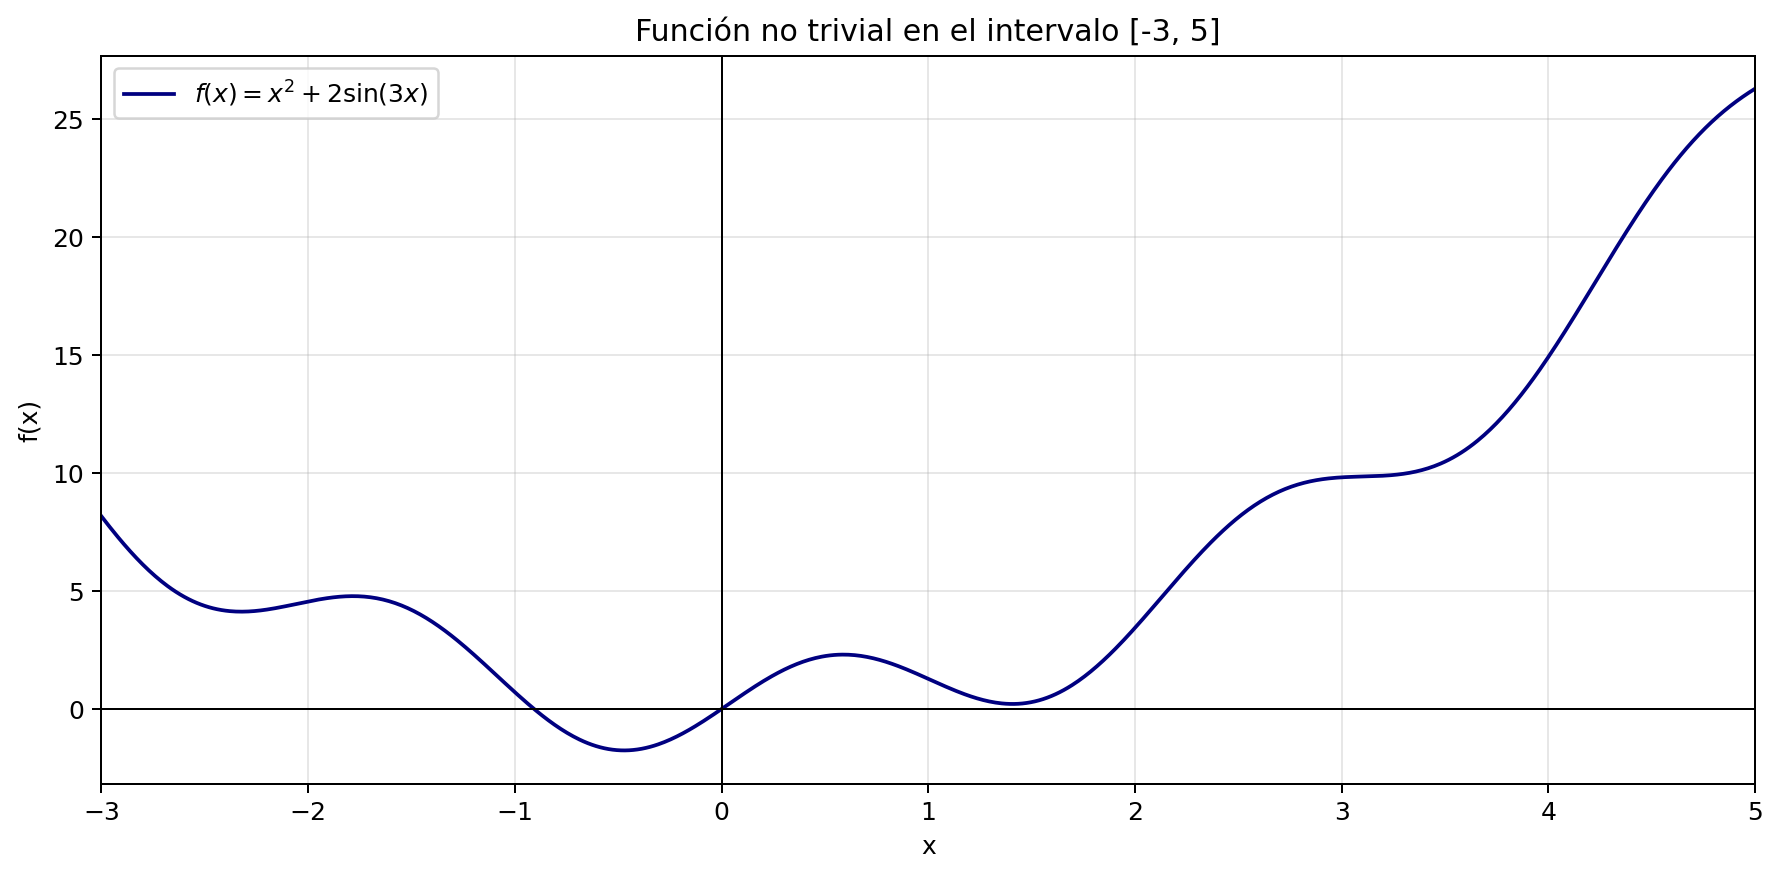
\includegraphics[width=0.9\textwidth]{figura_parte3.png}
\caption{Gráfica de $f(x)=x^2+2\sin(3x)$ en el intervalo $[-3,5]$.}
\label{fig:funcion-no-trivial}
\end{figure}

\subsection{Predicciones}

Las siguientes predicciones se formularon antes de ejecutar los algoritmos, utilizando la gráfica, el signo de $f'$ en puntos relevantes y la dirección del primer paso de cada método. Por este motivo son cualitativas; las aproximaciones numéricas se presentan recién en la sección de resultados.

\textbf{Bisección}

En el intervalo $[-2,1]$ hay más de un punto crítico. El primer punto medio es $-0.5$ y, como $f'(-2)>0$ y $f'(-0.5)<0$, se supone que las primeras subdivisiones conservarían la parte negativa del intervalo y llevarían al máximo local visible. En $[-1,0]$, $f'$ cambia de negativa a positiva, por lo que se espera encontrar un mínimo local dentro del intervalo. En $[1,2]$ ocurre el mismo cambio de signo y espera también un mínimo local.

\textbf{Newton}

Desde $x_0=-2$ esperamos que la convergencia al máximo local próximo se observa en la zona negativa. Desde $x_0=-1$, el signo y la magnitud del primer paso llevan la aproximación hacia la zona positiva, por lo que se esperó llegar al máximo local visible en esa región. Desde $x_0=4$ no se esperó una convergencia confiable, ya que el punto está lejos de los extremos visibles y la curvatura cambia durante las iteraciones.

\textbf{Descenso por gradiente}

Para la comparación principal se utilizó $\alpha=0.05$. Como $f'(-3)<0$, desde $x_0=-3$ el primer paso avanza hacia la derecha y se espera una convergencia al primer mínimo local visible. El valor $x_0=0.585$ se encuentra apenas a la izquierda de un máximo y tiene derivada positiva, por lo que el descenso comienza hacia la izquierda. Como $f'(4)>0$, desde $x_0=4$ el método también comienza hacia la izquierda y se supone una convergencia al mínimo local visible en la zona positiva.

\subsection{Resultados}

Después de ejecutar cada método con las condiciones iniciales indicadas, se obtuvieron los resultados de la Tabla \ref{tab:resultados-parte3}. Los métodos se ejecutaron con tolerancia interna $10^{-8}$ y un máximo de 1000 iteraciones. Además, un resultado sólo se consideró convergente cuando terminó antes del máximo de iteraciones y cumplió $|f'(x)|<10^{-6}$. La clasificación se realizó evaluando el signo de $f''$ en cada aproximación convergente.

\begin{table}[h]
\centering
\resizebox{\textwidth}{!}{%
\begin{tabular}{lllrrlll}
\hline
Método & Condición & Predicción & Aproximación & Iteraciones & $|f'(x)|$ & Estado & Clasificación \\
\hline
Bisección & $[-2,1]$ & Máximo local en la zona negativa & $-1.782932473$ & 29 & $2.345\cdot10^{-8}$ & Converge & Máximo local \\
Bisección & $[-1,0]$ & Mínimo local dentro del intervalo & $-0.471043177$ & 27 & $1.198\cdot10^{-7}$ & Converge & Mínimo local \\
Bisección & $[1,2]$ & Mínimo local dentro del intervalo & $1.407956578$ & 27 & $2.235\cdot10^{-8}$ & Converge & Mínimo local \\
Newton & $x_0=-2$ & Máximo local próximo al inicio & $-1.782932475$ & 6 & $8.882\cdot10^{-16}$ & Converge & Máximo local \\
Newton & $x_0=-1$ & Máximo local en la zona positiva & $0.589531341$ & 6 & $6.661\cdot10^{-16}$ & Converge & Máximo local \\
Newton & $x_0=4$ & No se espera convergencia & $7.820891884$ & 1000 & $1.505\cdot10^{1}$ & No converge & No corresponde \\
Gradiente & $x_0=-3$, $\alpha=0.05$ & Mínimo local hacia la derecha & $-2.322807411$ & 16 & $5.333\cdot10^{-8}$ & Converge & Mínimo local \\
Gradiente & $x_0=0.585$, $\alpha=0.05$ & Mínimo local hacia la izquierda & $-0.471043171$ & 15 & $4.856\cdot10^{-10}$ & Converge & Mínimo local \\
Gradiente & $x_0=4$, $\alpha=0.05$ & Mínimo local hacia la izquierda & $1.407956578$ & 32 & $1.664\cdot10^{-8}$ & Converge & Mínimo local \\
\hline
\end{tabular}
}
\caption{Resultados de los métodos para $f(x)=x^2+2\sin(3x)$.}
\label{tab:resultados-parte3}
\end{table}

Bisección y descenso por gradiente coincidieron con todas las predicciones. Newton también tuvo el comportamiento previsto. Desde $x_0=4$ alcanzó el máximo de iteraciones con residuo $|f'(x)|\approx15.047$. El último valor devuelto no es un punto crítico, aunque el método siempre devuelve una aproximación al finalizar.

\subsection{Comparación de learning rates}

Se probaron cuatro valores de $\alpha$ con las tres condiciones iniciales del descenso por gradiente. Para que la comparación fuera válida se utilizó una variante con la misma actualización del método original, pero con el criterio común $|f'(x_{k+1})|<10^{-6}$. De esta manera la tolerancia no depende del tamaño del learning rate.

\begin{table}[h]
\centering
\resizebox{\textwidth}{!}{%
\begin{tabular}{ccrrrll}
\hline
$\alpha$ & $x_0$ & Último $x$ & $|f'(x)|$ & Iteraciones & Estado & Clasificación \\
\hline
0.01 & $-3$ & $-2.322807474$ & $8.896\cdot10^{-7}$ & 108 & Converge & Mínimo local \\
0.01 & $0.585$ & $-0.471043124$ & $9.215\cdot10^{-7}$ & 109 & Converge & Mínimo local \\
0.01 & $4$ & $1.407956628$ & $9.289\cdot10^{-7}$ & 202 & Converge & Mínimo local \\
0.05 & $-3$ & $-2.322807444$ & $4.884\cdot10^{-7}$ & 14 & Converge & Mínimo local \\
0.05 & $0.585$ & $-0.471043169$ & $4.350\cdot10^{-8}$ & 14 & Converge & Mínimo local \\
0.05 & $4$ & $1.407956585$ & $1.581\cdot10^{-7}$ & 31 & Converge & Mínimo local \\
0.10 & $-3$ & $-2.322807438$ & $4.126\cdot10^{-7}$ & 17 & Converge & Mínimo local \\
0.10 & $0.585$ & $-0.471043221$ & $9.985\cdot10^{-7}$ & 612 & Converge & Mínimo local \\
0.10 & $4$ & $1.407956531$ & $8.106\cdot10^{-7}$ & 63 & Converge & Mínimo local \\
0.20 & $-3$ & $0.337657079$ & $3.851$ & 1000 & No converge & No corresponde \\
0.20 & $0.585$ & $0.289579873$ & $4.454$ & 1000 & No converge & No corresponde \\
0.20 & $4$ & $0.018374947$ & $6.028$ & 1000 & No converge & No corresponde \\
\hline
\end{tabular}
}
\caption{Comparación de learning rates para descenso por gradiente.}
\label{tab:learning-rates}
\end{table}

Con $\alpha=0.01$ se obtuvieron los tres mínimos esperados en 108, 109 y 202 iteraciones. El valor $\alpha=0.05$ produjo las menores cantidades de iteraciones entre los valores probados, con 14, 14 y 31. Con $\alpha=0.10$, el caso $x_0=0.585$ necesitó 612 iteraciones. Cerca del mínimo $x\approx-0.471$ se tiene $f''(x)\approx19.777$, por lo que las aproximaciones oscilan y el residuo disminuye lentamente. Con $\alpha=0.20$ ninguno de los tres casos cumplió el criterio de residuo en 1000 iteraciones. Los residuos finales quedaron entre $3.851$ y $6.028$, por lo que esos valores no son puntos críticos.

\subsection{Preguntas de la sección 3.3}

\textbf{¿Los métodos funcionaron como se esperaba para las condiciones iniciales?}

Sí. Ocho casos convergieron a los puntos previstos y el caso restante tuvo la falta de convergencia esperada. El resultado más sensible fue Newton desde $x_0=4$, que terminó en $x=7.820891884$ con residuo $15.047146$. También se observó que un intervalo de bisección puede contener varios puntos críticos. En ese caso el resultado depende de las subdivisiones que produce el algoritmo.

\textbf{¿Cómo se puede usar descenso por gradiente para obtener máximos sin cambiar el algoritmo?}

Se puede aplicar el mismo algoritmo a la función $-f$. Un mínimo de $-f$ corresponde a un máximo de $f$. La Tabla \ref{tab:maximos-parte3} muestra el experimento con $\alpha=0.05$ y criterio de residuo $10^{-6}$.

\begin{table}[h]
\centering
\resizebox{\textwidth}{!}{%
\begin{tabular}{crrrrll}
\hline
$x_0$ & Último $x$ & $f(x)$ & $|f'(x)|$ & Iteraciones & Estado & Clasificación para $f$ \\
\hline
$-3$ & $-4.780552\cdot10^8$ & $2.285368\cdot10^{17}$ & $9.561\cdot10^8$ & 200 & No converge & No corresponde \\
$0.585$ & $0.589531319$ & $2.308551$ & $3.533\cdot10^{-7}$ & 8 & Converge & Máximo local \\
$4$ & $7.272879\cdot10^8$ & $5.289477\cdot10^{17}$ & $1.455\cdot10^9$ & 200 & No converge & No corresponde \\
\hline
\end{tabular}
}
\caption{Descenso por gradiente aplicado a $-f$ para buscar máximos de $f$.}
\label{tab:maximos-parte3}
\end{table}

Desde $x_0=0.585$ se obtuvo $x=0.589531319$ en 8 iteraciones, con residuo $3.533\cdot10^{-7}$. Este punto es un máximo local de $f$ porque $f''(0.589531319)<0$.

\textbf{¿Hay riesgo de que no converja la búsqueda de máximos?}

Sí. La función $f(x)=x^2+2\sin(3x)$ no está acotada superiormente cuando aumenta $|x|$. En consecuencia, $-f$ no está acotada inferiormente. Desde $x_0=-3$ y $x_0=4$ las aproximaciones alcanzaron magnitudes cercanas a $4.78\cdot10^8$ y $7.27\cdot10^8$ después de 200 iteraciones. Los residuos fueron del orden de $10^9$. Esto muestra que el método puede alejarse de los máximos locales y divergir.

\subsection{Conclusión}

Los experimentos muestran que la condición inicial y los parámetros del método son importantes cuando una función tiene varios extremos locales. Bisección fue estable en los intervalos elegidos y Newton fue rápido cuando convergió. El descenso por gradiente encontró los mínimos esperados con $\alpha=0.05$, mientras que $\alpha=0.20$ produjo inestabilidad. La búsqueda de máximos mediante $-f$ funcionó cerca de un máximo local, pero también mostró riesgo de divergencia debido al crecimiento de la función.

\end{document}
